% =========================================================================
% PÔSTER CIENTÍFICO (SIMPÓSIO DE INICIAÇÃO CIENTÍFICA UFABC)
% =========================================================================
\documentclass[final]{article}

\usepackage[utf8]{inputenc}
\usepackage[T1]{fontenc}
\usepackage[brazilian]{babel}

\IfFileExists{FiraSans.sty}{
    \usepackage[sfdefault,scaled=0.96]{FiraSans}
}{
    \usepackage[scaled=0.95]{helvet}
    \renewcommand{\familydefault}{\sfdefault}
}
\IfFileExists{newtxsf.sty}{
    \usepackage{newtxsf}
}{}

\usepackage[paperwidth=90cm, paperheight=120cm, margin=0cm]{geometry}
\usepackage{amsmath, amssymb, amsfonts}
\usepackage{booktabs}
\usepackage{array}
\usepackage{graphicx}
\usepackage[export]{adjustbox}
\usepackage{xcolor}
\usepackage{tikz}
\usepackage{enumitem}
\usepackage{ragged2e}
\usepackage{textcomp}
\usepackage{hyperref}

\DeclareUnicodeCharacter{00BA}{\textordmasculine}
\DeclareUnicodeCharacter{00AA}{\textordfeminine}

\graphicspath{
    {poster/logos/}
    {poster/images/}
    {figures/}
}

\definecolor{ufabcgreen}{HTML}{006633}
\definecolor{textdark}{HTML}{141414}

\hypersetup{
    colorlinks=true,
    urlcolor=ufabcgreen,
    linkcolor=ufabcgreen
}

\pagestyle{empty}
\setlength{\parindent}{0pt}
\setlength{\parskip}{0.42em}

\newcommand{\destaque}[1]{\textcolor{ufabcgreen}{\textbf{#1}}}

\newcommand{\postersection}[1]{
    \par\vspace{0.55em}
    {\fontsize{34}{40}\selectfont\bfseries\color{textdark}#1}
    \par\vspace{0.2em}
}

\newcommand{\postercaption}[2]{
    \par\vspace{0.22em}
    {\fontsize{25}{30}\selectfont\raggedright\textbf{#1:} #2\par}
    \vspace{0.3em}
}

\begin{document}
\color{textdark}
\fontsize{29}{35}\selectfont

% =========================================================================
% CABEÇALHO, FAIXA DE AUTORES E RODAPÉ
% =========================================================================
\begin{tikzpicture}[remember picture, overlay, shift={(current page.north west)}, inner sep=0pt, outer sep=0pt]

    \fill[ufabcgreen] (4.25cm, 0cm) -- (56.45cm, 0cm) -- (56.45cm, -8cm)
        arc[start angle=0, end angle=-90, radius=4cm] -- (8.25cm, -12cm)
        arc[start angle=-90, end angle=-180, radius=4cm] -- cycle;

    \node[anchor=center, text=white, text width=62cm, align=center] at (30.35cm, -6.0cm) {
        {\fontsize{58}{68}\selectfont\bfseries
        @@RESEARCH-TITLE@@:\\[0.18em]
        @@RESEARCH-SUBTITLE@@}
    };

    \node[anchor=south] at (66.0cm, -11.8cm) {
        
\includegraphics[width=13.0cm, height=10.8cm, keepaspectratio]{ufabc.png}
    };
    \node[anchor=south] at (81.2cm, -11.8cm) {
        
\includegraphics[width=13.0cm, height=10.8cm, keepaspectratio]{uscs.png}
    };

    \node[anchor=north, text width=84.8cm, align=center] at (45.0cm, -12.5cm) {
        {\fontsize{31}{37}\selectfont\bfseries @@AUTHOR@@, @@ADVISOR@@}\\[0.2em]
        {\fontsize{28}{33}\selectfont
        Centro de Matemática, Computação e Cognição -- Universidade Federal do ABC\\[0.08em]
        Av. dos Estados, 5001 -- Bangú, Santo André - SP}
    };

    \node[anchor=north west] at (1.3cm, -111.3cm) {
        {\fontsize{30}{36}\selectfont\bfseries Apoio:}
    };

    \node[anchor=center] at (2.7cm, -114.7cm) {
        
\includegraphics[height=3.2cm, keepaspectratio]{ufabc.png}
    };
    \node[anchor=center] at (6.5cm, -114.7cm) {
        
\includegraphics[width=3.9cm, keepaspectratio]{uscs.png}
    };
    \node[anchor=center] at (4.6cm, -118.0cm) {
        
\includegraphics[width=6.6cm, keepaspectratio]{cnpq.png}
    };
    \node[anchor=center] at (13.7cm, -115.8cm) {
        
\includegraphics[width=7.6cm, keepaspectratio]{toca.png}
    };

    \begin{scope}
        \clip (18.4cm, -120.0cm) rectangle (90.0cm, -110.8cm);
        \fill[ufabcgreen] (18.4cm, -120.0cm) rectangle (90.0cm, -110.8cm);
        \node[anchor=center, opacity=0.35] at (36.2cm, -115.4cm) {
            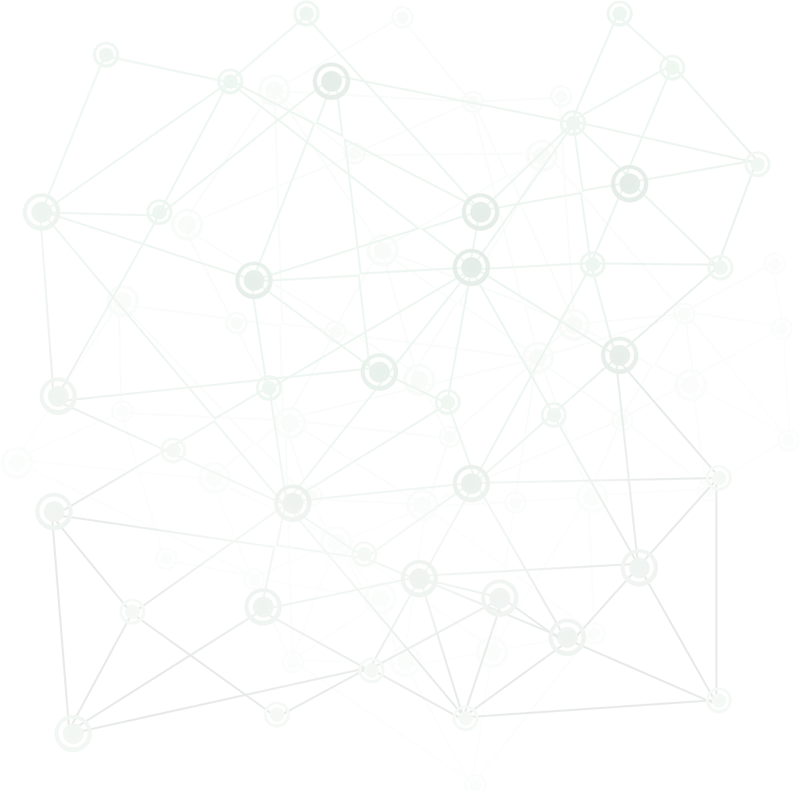
\includegraphics[width=36.0cm]{background.png}
        };
    \end{scope}

    \node[anchor=east, align=right, inner sep=0pt] at (88.4cm, -115.4cm) {
        {\fontsize{80}{92}\selectfont\bfseries\color{white}\mbox{Encontro de Iniciação Científica}}\\[0.22em]
        {\fontsize{40}{48}\selectfont\bfseries\color{white}\mbox{Simpósio de Iniciação Científica da UFABC}}\\[0.15em]
        {\fontsize{40}{48}\selectfont\bfseries\color{white}\mbox{@@YEAR@@}}
    };

\end{tikzpicture}

% =========================================================================
% CORPO PRINCIPAL
% =========================================================================
\vspace*{18.0cm}
\noindent
\hspace*{2.6cm}
\begin{minipage}[t]{41.275cm}
\justifying
\setlength{\parindent}{0pt}
\setlength{\parskip}{0.38em}

\postersection{INTRODUÇÃO}
@@RESEARCH-DESC@@

\vspace{0.18em}
\noindent
\setlength{\fboxrule}{0.12em}
\fcolorbox{textdark}{white}{
    \begin{minipage}{\dimexpr\linewidth-0.84em-0.24em\relax}
        \vspace{0.18em}
        \fontsize{23}{27}\selectfont\raggedright
        \destaque{Formulação do Problema Base}\\[0.10em]
        \textbf{Entrada:} Instância $I$ do domínio investigado.\\[0.08em]
        \textbf{Saída:} Solução exata certificada segundo o critério de otimalidade.
    \end{minipage}
}
\vspace{0.18em}

\postersection{FUNDAMENTAÇÃO TEÓRICA E ARQUITETURA C++23}
\begin{itemize}[leftmargin=1.2em, itemsep=0.18em, topsep=0.1em]
    \item \destaque{Teorema Central:} Enuncie aqui o principal resultado estrutural ou dualidade da pesquisa [1].
    \item \destaque{Arquitetura Polimórfica:} Classes base abstratas em \textbf{C++23} com separação limpa entre interface (\texttt{AlgorithmBase}) e motores concretos.
\end{itemize}

\vspace{0.15em}
{\fontsize{24}{29}\selectfont
\renewcommand{\arraystretch}{1.15}
\setlength{\tabcolsep}{6pt}
\begin{tabular*}{\linewidth}{@{\extracolsep{\fill}}llr@{}}
\toprule
\textbf{Classe C++23} & \textbf{Paradigma} & \textbf{Complexidade} \\
\midrule
\texttt{AlgorithmBase} & Interface abstrata & --- \\
\destaque{SampleAlgorithm} & Motor de referência inicial & $\mathcal{O}(n)$ \\
\bottomrule
\end{tabular*}
}
\postercaption{Tabela 1}{Arquitetura base de algoritmos implementados em C++23.}

\postersection{APLICAÇÃO PRÁTICA}
Espaço reservado para a formulação e resultados visuais da aplicação principal desenvolvida na pesquisa.

\end{minipage}
\hspace{2.25cm}
\begin{minipage}[t]{41.275cm}
\justifying
\setlength{\parindent}{0pt}
\setlength{\parskip}{0.38em}

\postersection{RESULTADOS EXPERIMENTAIS}
Os experimentos comparam os motores implementados sobre instâncias padronizadas e sintéticas com medição isolada de tempo de CPU via \texttt{std::chrono} e validação cruzada de corretude.

\vspace{0.3em}
\begin{center}
\begin{tikzpicture}
    \draw[line width=2pt, draw=ufabcgreen, fill=gray!8, rounded corners=8pt] (0, 0) rectangle (38cm, 16cm);
    \node[font=\fontsize{28}{34}\selectfont\bfseries, text=textdark] at (19cm, 8cm) {Espaço reservado para gráficos e curvas de escalabilidade};
\end{tikzpicture}
\end{center}
\postercaption{Figura 1}{Comparação de desempenho e escalabilidade assintótica.}

\vspace{0.15em}
{\fontsize{24}{29}\selectfont
\renewcommand{\arraystretch}{1.16}
\setlength{\tabcolsep}{5pt}
\begin{tabular*}{\linewidth}{@{\extracolsep{\fill}}lrr@{}}
\toprule
\textbf{Instância} & \textbf{Tamanho} & \textbf{Tempo Médio (ms)} \\
\midrule
\texttt{sample\_01} & 1.000 & \destaque{0,01} \\
\texttt{sample\_05} & 5.000 & \destaque{0,04} \\
\bottomrule
\end{tabular*}
}
\postercaption{Tabela 2}{Síntese inicial de medições experimentais.}

\postersection{AGRADECIMENTOS}
Projeto desenvolvido na UFABC (Edital @@EDITAL@@). Repositório público em C++23: \url{https://github.com/@@GITHUB-USER@@/@@RESEARCH-SLUG@@}.

\postersection{BIBLIOGRAFIA}
{\fontsize{25}{30}\selectfont
\begin{enumerate}[label={[\arabic*]}, leftmargin=1.8em, itemsep=0.18em, topsep=0.1em]
    \item CORMEN, T.\ H. et al. \textbf{Introduction to Algorithms}. 4th ed. MIT Press, 2022.
    \item KORTE, B.; VYGEN, J. \textbf{Combinatorial Optimization}. 6th ed. Springer, 2018.
\end{enumerate}
}

\end{minipage}

\end{document}
